\section{Introduction}
This course teaches architectural styles and patterns, methods for constructing and evaluating architectures, and component-based development. Design patterns and object-oriented frameworks are also covered. \\

The goal of this project is to develop a fully functional two player version of the classic board game \emph{Nine Men's Morris}, using the methods and styles in accordance with the course goals. \\

The second chapter of this document covers the functional requirements of the application. The third chapter concerns the quality requirements, while the fourth chapter covers COTS components and technical constraints. Chapter five and six covers issues and document changes, respectively, and is followed by the document's references.



\subsection{Concept}

\begin{wrapfigure}{r}{0.5\textwidth}
  \begin{center}
  \vspace{-32pt}
    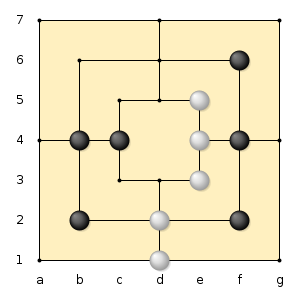
\includegraphics[width=0.48\textwidth]{concept2.png}
  \end{center}
  \vspace{-20pt}
  \caption{Game concept}
  \vspace{1pt}
\end{wrapfigure}

The game is based on the concept of \emph{Nine Men's Morris}, and is developed by Ole Jørgen Rishoff, Stian Sørebø, Emil Andreas Mork, and Steinar Haram. It is an abstract strategy board game for two players that emerged from the Roman Empire. Each player has nine pieces, or "men", that move among the board's twenty-four spots. The goal of the game is to leave the opposing player with fewer than three pieces or, as in checkers, no legal moves. The way to remove one of the components pieces, is to get your own pieces in a three in a row position. The functional requirements in the next section will reflect these game rules, and also cover other more specific scenarios. 



